\documentclass[runningheads]{llncs}

\usepackage[T1]{fontenc}
\usepackage{graphicx}
\usepackage{comment}

% Packages
\usepackage[dvipsnames,svgnames]{xcolor} % text color
\usepackage[normalem]{ulem} % wavy underlines

% Comments
\newcommand{\todo}[1]{\noindent\textcolor{red}{{\bf \{TODO}: #1{\bf \}}}}
\newcommand{\TODO}[1]{\todo{#1}}
\newcommand{\citeneeded}{\textcolor{red}{{\bf [?!]}}}
\newenvironment{draft}{\color{gray}}{\color{black}}

% Reviewers
\newcommand\rv[1]{{\color{RubineRed}\textbf{RV}: #1}}
\newcommand\rt[1]{{\color{Red}\textbf{RT}: #1}}

% Annotations
\makeatletter
\font\uwavefont=lasyb10 scaled 700
\def\spelling{\bgroup\markoverwith{\lower3.5\p@\hbox{\uwavefont\textcolor{Red}{\char58}}}\ULon}
\def\grammar{\bgroup\markoverwith{\lower3.5\p@\hbox{\uwavefont\textcolor{LimeGreen}{\char58}}}\ULon}
\def\phrasing{\bgroup\markoverwith{\lower3.5\p@\hbox{\uwavefont\textcolor{RoyalBlue}{\char58}}}\ULon}
\let\rephrase\phrasing
\newcommand\remove{\bgroup\markoverwith{\textcolor{red}{\rule[0.5ex]{2pt}{0.4pt}}}\ULon}
\newcommand\insertion{\bgroup\markoverwith{\textcolor{Green}{\rule[-0.5ex]{2pt}{0.6pt}}}\ULon}
\makeatother


\begin{document}

\title{PErsoNal Genome QUery IN healthcare and clinical practice (PENGQUIN)}

\author{Elias Crum\inst{1,2}\orcidID{0009-0005-3991-754X}}

\authorrunning{E. Crum}
\institute{IDLab, Department of Electronics and Information Systems, Ghent University -- imec, Belgium \and Flemish institute for Technological Research (VITO) Mol, Belgium}


\maketitle

\begin{abstract}
	Medical care is in the process of becoming increasingly personalized through the use of patient genetic information. 
	At present, digital data useful for clinical care is commonly diffuse, organized arbitrarily, and stored in data silos. 
  \phrasing{Here I propose an early stage Ph.D.} that aims to improve shareability of genomic data storage(s), while preserving data privacy, through the use of Solid pods. 
  \rv{What is the \emph{problem} though? Above only lists cause and proposed solution.}
	I also propose plans to investigate representing personal genome sequence data in Resource Description Format as Linked Data, where linkages are representative of semantic, medically relevant data.
	To make such a storage framework clinically useful, I aim to evaluate the how queries over this Linked genomic Data could be executed using a query engine approach.
  \rv{Still missing problem.}
	Preliminarily, I have succeeded in storing genomic data in representative patient data pods using Solid specifications. 
	I aim to show in future work that this novel approach to storing clinical patient genomic data improves clinical data shareability, discoverability, and data flow efficiency through the use of Linked Data formats and querying infrastructure. 

\keywords{Solid \and Linked Data \and Querying \and Genomic Data Sharing}

\end{abstract}


\section{Introduction / Motivation}
\begin{comment}
Give a general introduction to the domain/area/topic and indication of its importance/impact in Semantic Web research or other domains.
\end{comment}

As our understanding of genomics deepens, the role of Personal Genome Sequencing (PGS) in healthcare is expanding. 
At the time of writing, there are multiple domains of clinical practice where patient PGS data is now used to inform medical decision making \cite{souche_recommendations_2022,gil_analysis_2015}. 
Despite recent advances, PGS data usage has yet to be scaled to more generalized clinical practice \cite{alzubi_personal_2014}. 
While there are many documented challenges to wider clinical implementation of PGS data~\cite{stefanicka-wojtas_barriers_2023}, one major challenge is presented by the digital representation, storage, and access to the PGS data that underlies established medical workflows.
With the PENGQUIN project, I aim to address the challenges presented by PGS data usage in clinical practice by leveraging  decentralized storage, data representation, and querying technologies.  

\rv{Remember that you're not writing for medical experts here. Could you incorporate an example above of how decision making is informed?}

\subsubsection{Medical Motivations for PGS data in Clinical Practice}
At present, there are major medical fields that preliminarily show readiness for greater use of PGS data, these being drug development and prescription, cancer diagnosis and treatment, and rare genetic disease identification and treatment.
Genomic variation is thought to account for up to 95\% of outcome variations in drug prescription and treatment efficacy~\cite{belle_genetic_2008}, while also becoming informative for new drug development recently \cite{ko_new_2022}. 
In clinical practice, studies have documented genotype correlation with unintended drug responses for commonly prescribed drugs such as warfarin \cite{linder_genetic_2001} and many others \cite{research_table_2024}. 
PGS usage, by helping predict, better understand, and inform optimal drug treatment plans, shows great potential for improving on the one-size-fits-all, trial and error approach to drug prescription popularly practiced today \cite{hens_return_2011}. 
Similarly, for cancer patients, the use of PGS data has been shown to augment existing strategies of diagnosis and treatment \cite{mcleod_cancer_2013}. 
One of the most developed, wide-spread implementations of PGS data usage in clinical practice currently is in rare genetic disease identification and treatment \cite{krier_genomic_2016}. 
Despite these advanced use cases, barriers to adoption remain, especially due to the cost and technological infrastructure demands posed by large scale PGS data generation, storage, and analysis.

\rv{This medical background should probably be shortened for the target audience; does not need as many domain references.}

\subsubsection{PGS data storage and sharing} 
PGS data are expensive to both generate and store. 
The average human genome is slightly over 3 billion base pairs in length (3 Gbp). 
During a whole genome sequencing workflow, various sequence formats, that offer different sets of information, such as FASTQ \cite{cock_sanger_2010}, SAM/BAM/CRAM \cite{li_sequence_2009}\cite{bonfield_cram_2022}, VCF \cite{danecek_variant_2011}, and others are produced and stored indefinitely. 
VCF files are typically between 100-1000s MB (0.1-1 GB) within computer memory and represent around 3 million nucleotide positions of an individual's PGS. 
VCF file format serve as the state-of-the-art for most clinical genomic applications.

\rv{The above paragraph is a good example of what the target audience needs to know.}

For these genomic data, along with the financial considerations, there are also significant privacy considerations.
Unfortunately, this relationship between privacy and cost is largely antagonistic within the current technological framework.
Increases in privacy protections for PGS data often lead to increases in data siloing and increased general costs for both patient and provider.
To make PGS data usage in healthcare more scalable, decreases in costs and preservation, or improvement of, current privacy standards for PGS data storage are required.

One strategy that could reduce costs is the increase of data sharing and discoverability between hospital systems.
\rv{Okay, this is the essence---that should definitely make it into the abstract!}
The increase in data sharing could be further augmented by greater connectivity of a single patient's data, such as previous test results, PGS data, medical history, etc.
Increasing patient data connectedness and accessibility for authorized users is not a trivial problem while also maintaining privacy.
It is at this crossroads that the current state-of-the-art in clinical data storage technology is largely incapable of achieving both goals.

\rv{Excellent paragraph}}

\subsubsection{Solid - A semantic alternative} 
A conceptual approach that offers solutions to the current dead-end described above is a citizen-centric system of clinical PGS data storage. 
The citizen-centric model places the patient at the center, and is not an entirely novel concept [c].
To accomplish a citizen-centric storage approach, the Solid protocol \cite{capadisli_solid_nodate}, offers the foundation for building a framework to granularize data privacy, allow authorized data access over the web, represent stored data as Linked Data, among others. 
While there is still much work to be done before this fledgling technologies can be applied to clinical practice, Solid provides the foundational components to build a citizen-centric storage framework, thereby, removing some of the antagonism between cost reduction and privacy.

\rv{The title of the paragraph mismatches with its contents; if the title is correct, what is the benefit of semantics?}

\textbf{Resource Description Format and Linked Data.}
To fully harness the advantages offered by Solid, experimentation with semantic data representation and data linkages hold great promise to both reduce costs and improve medical efficacy.
Resource Description Framework (RDF) is a way of semantically representing data that also allows for data linking across documents and datastores.
Some large public biological databases, such as UniProt \cite{theuniprotconsortium_uniprot_2017}, have been fully converted to RDF and initiatives exist for further expansion of biological data storage as RDF \cite{sib_swiss_institute_of_bioinformatics_rdf_group_members_sib_2024}.
RDF holds promise within healthcare for connecting clinically-relevant data and has been proposed for use in Electronic Patient Records in the past \cite{lindemann_resource_2008}.
More modernly, initiatives for improving the interoperability of health data through integrating semantic layers of information into data stores, primarily through the representation of data as RDF, have been undertaken in Europe \cite{van_der_horst_bridging_2023}.
With more and more data being represented in RDF, the advantages of such a data formatting strategy are now becoming increasingly possible.

\rv{Well yes, but for our target audience, make this more tangible. They know RDF already; the biological data argument is good, but the rest of the paragraph needs to be more tangible. It's currently more at the level for that medical professionals need to know.}

\textbf{Project Motivation.}
Despite there being no real solutions to the current antagonism between privacy and cost reduction for PGS data usage in healthcare, there is also a conspicuous gap in the current scientific discourse around the development and implementation of a proposed solution. 
This gap underscores the necessity of my research project.
My aim is to develop a framework for storing, sharing, linking, and querying PGS data in Patient Genome Pods using the Solid protocol \cite{capadisli_solid_nodate}.
My project described here will aim to establish a proof-of-concept demonstration of how a decentralized storage framework for PGS data could achieve both cost reduction goals along with privacy protections.


\section{State of the Art}
\begin{comment}
Describe existing work in the area, work focusing on the same/similar problems or that might be useful to tackling your research question.
\end{comment}

\subsection{Current State of the Art -- Clinical data storage}
Presently, most clinically relevant health data is stored using an \textbf{institution-centric approach}, including PGS data. 
This strategy is characterized by the hospital or hospital system isolating all of its stored data into one or more centralized databases that are governed and maintained solely by the owner institution. 
Here, centralized storage is defined as the structural organization of a data store, establishing that a single node, the system that hosts the physical data storage, has control over managing database content, access, and permissions. 
With this system, healthcare institutions prioritize patient data privacy over all other digital data storage considerations. 
By prioritizing patient data privacy, access is commonly only allowed for authorized users within the institution\textquotesingle s internal network. 
Crucially, this institution-centric data storage architecture, by design, allows for little to no accessibility for users or data usage requests that originate outside of the institution\textquotesingle s network, largely due to the organizational design of such centralized data storage systems. 
With the enlarged threat of hacking, phishing, and login credential compromisation that seems to only be increasing \cite{noauthor_ransomware_nodate}, hospitals and institutions that maintain patient PGS data are forced to enact tighter regulation over data access within their institution, severely limit outside institution access, and increase the in-house cyber security staff or pay for external companies to handle such security audits.  
Due to this isolation of patient PGS data to a single institution, data duplication leading to increased storage and data generation costs, severely limited patient data usage transparency, and severely limited potential for data sharing are observed. 
Collectively, these state-of-the-art approaches to PGS data storage inhibit the scalability of PGS data usage in the above discussed clinical applications due to raising PGS usage costs.

\subsubsection{Current State of the Art -- Academic Reserach and Consumer Market}
Apart from the current practices within healthcare institutions, other approaches for consumer access to their PGS data by private companies, PGS data sharing between research institutions, and general health data interoperability initiatives by multi-institution consortiums have been innovating the ways PGS data is stored and shared. 

Private companies, such as 23andMe, Ancestry.com, Sequencing.com, and others, offer consumption-centered genomic products such as ancestry profiles, health risk screenings, and rare-disease management guidelines among other emerging services. 
Such services have highlighted a public interest in being able to see and access their PGS data as well as learn useful things about themselves from it.
At the same time, innovation in this niche is not situated to handle the challenges presented by PGS data in clinical practice while also utilizing similar centralized data storage approaches to hospital systems.

In the realm of academic research, the development of infrastructure that allows for sharing of genome data between institutions has gained traction recently. 
Initiatives such as GA4GH Beacons \cite{rambla_beacon_2022} and others are building infrastructure for between institution data sharing. 
The major drawbacks of these proposed solutions are, (a) the requirement that data is anonymized for true sharing or, (b) control of data analysis is relinquished to the data\textquotesingle s home institution, thereby establishing federated networks of hospital data for data discoverability, but restricting actual access to such data for privacy reasons.

Despite great progress in research and consumer domains, advancements in state-of-the-art infrastructure and standards are not directly translatable to clinical practice largely because clinical application was never their goal. 

\subsubsection{Solid, RDF, and Linked Data in clinical practice}
At present, there are initiatives pushing for the adoption of Solid technology for greater use within medical ..
One initiative of note is the WE ARE movement in Flanders that is developing an application for the request of consent ....

RDF ...

Linked Data ...

\textbf{Link Traversal Query Processing}
With the representation of PGS data as RDF, approaches to parsing and querying that data must also be investigated, especially to encourage leveraging the greatest utility from the linked nature of representing PGS data as Linked Data.
The querying of Linked Data is a well established challenge, especially for large datasets \cite{taelman_evaluation_2023}.
I forsee the main challenges posed by link traversal in general contexts as less daunting within our proposed framework because most work where significant challenges were observed were with generalized, web-scale querying \cite{taelman_evaluation_2023}. 
Here, I am proposing a relatively small number of links within a large, known dataset. 
Query processing over a large dataset is made more performant through following strategies such as query planning.
Query planning involves the maximization of query performance based on cost estimations based on data and query type. 
Additional underlying strategies such as the use of MapReduce frameworks for query execution optimization can also improve query performance through the use of query decomposition and parallel processing \cite{shim_mapreduce_2013}.  


\section{Problem Statement and Contributions}
\begin{comment}
Formulate the problem you intend to solve, and how you intend to contribute to Semantic Web research. This section should include a clear formulation of one (or very few) research hypothesis (what statement you want to validate through your methodology, approach and evaluation), and/or the research questions that need to be answered.
\end{comment}

My research project is situated to provide a proof-of-concept PGS data storage and sharing framework that can be adapted to use for clinical practice. 
In this pursuit, my core research questions are: 
(A) Can a citizen-centric PGS data storage framework, developed using a decentralized storage technology, offer data sharing infrastructure while maintaining privacy safeguards for sensitive data? 
(B) Can PGS data be stored as RDF, be linked to other medically-relevant data, and be queried over in a ways that would be useful to clinical practice.
To address these central questions, I will investigate the use of data pods, implemented using Solid protocol, to store PGS data in a decentralized and privacy-oriented ecosystem while addressing technical challenges associated with data policies, representation of PGS data as Linked Data, discoverability through querying, and infrastructure that connects data pods to existing clinical workflows and tools. 
My hypothesis is that such a framework can be developed and would offer unique advantages over the existing state-of-the-art institution-centric PGS data storage solutions. 

The following six objectives will be undertaken to test my hypotheses through experimental production and testing of different modules of the proposed framework.
\begin{enumerate}
    \item Solid Pod PGS Data Storage
    \item Genomic data as Linked Data
    \item Data policies and sharing infrastructure
    \item Data querying
    \item Framework deployment
\end{enumerate}

Together, these objectives will serve as the components of an operational framework that uses the proposed methods for storing, sharing, linking, and querying PGS data for clinical use. The framework, once produced, will be compared to existing strategies for storing and sharing PGS data to assess the efficacy of transitioning toward product production and marketing.

The proposed scientific approach will contribute novel data and conclusions to numerous fields of semantic web research. These findings will include an approach to how decentralized storage specifications can be applied to store sensitive medical data, how genomic and medical data can be represented and queried as Linked Data, how existing Linked Data querying algorithms perform over genomic and health data, how granularized data policies impact querying and linking data in a medical context, and how the combination of these semantic technologies could provide an improvement over existing state-of-the-art clinical PGS data storage and usage strategies, to just name a few.


\section{Research Methodology and Approach}
\begin{comment}
Describe the research methodology you will apply in your research, including the different steps from the formulation of your research questions to answering them. Also describe the approach you are taking (or you intend to take for Early Stage Ph.D. submissions) to instantiate the research methodology, hence contributing to solve the problem described in Section 3 and confirm or reject your hypothesis. Discuss how this approach is innovative and novel, and how it is (might be) implemented.
\end{comment}

My project will be split into four different component work packages and a final fifth work package where the components will be deployed as a cohesive framework within a web application. 

\begin{figure}
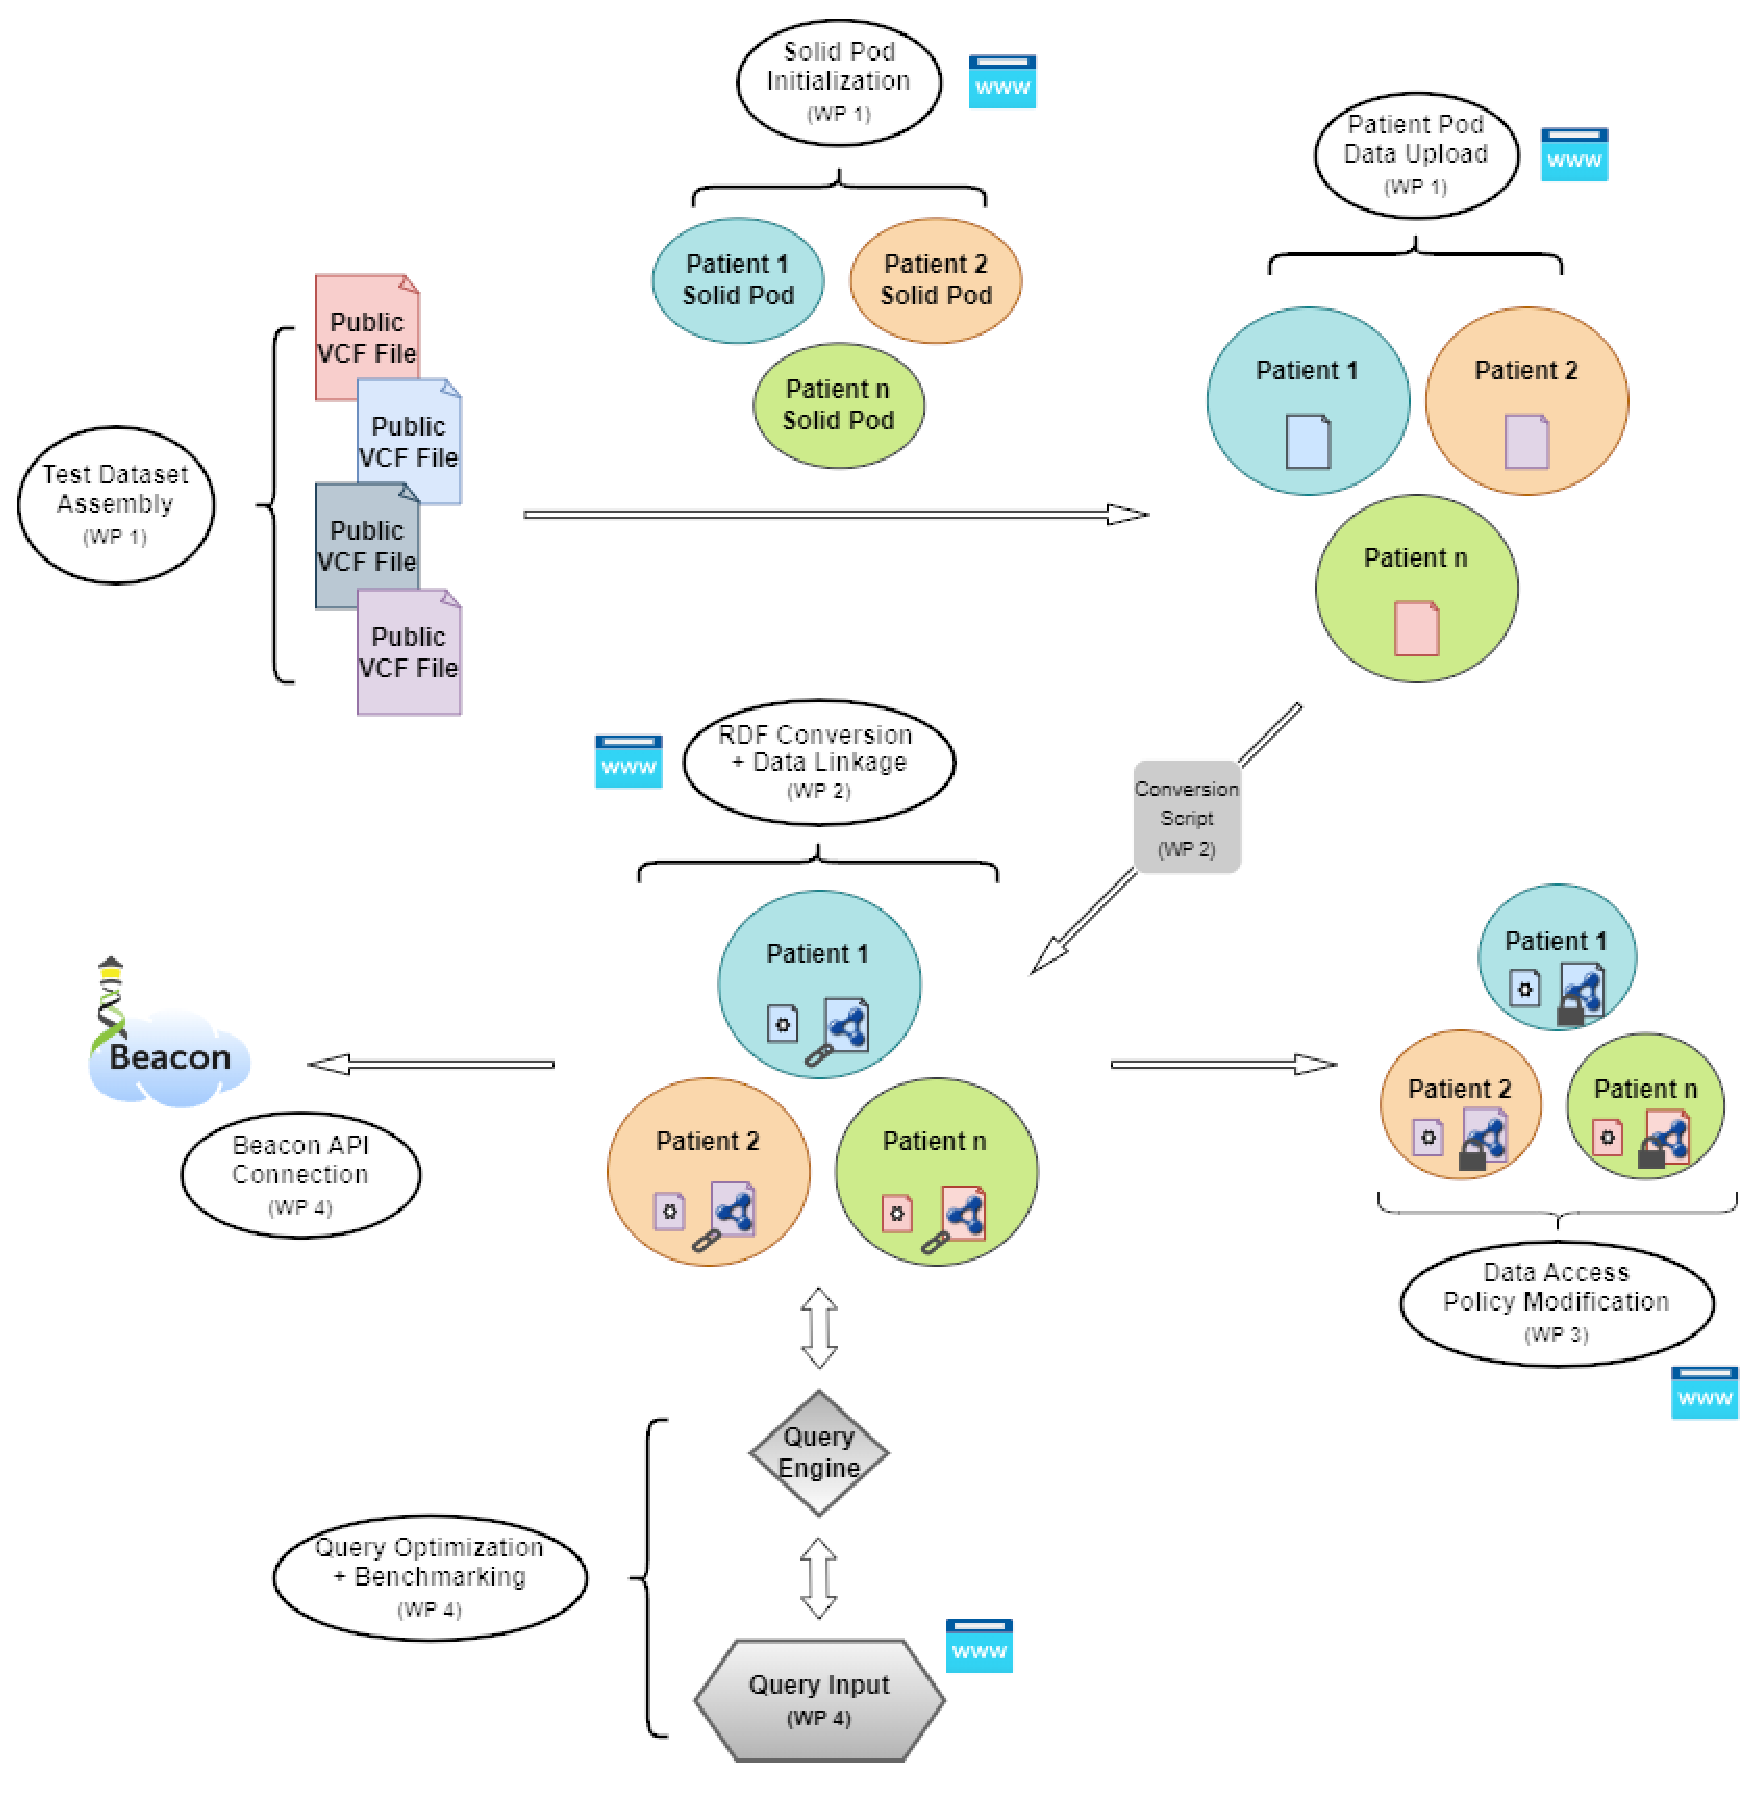
\includegraphics[width=\textwidth]{fig1.eps}
\caption{\textbf{PENGQUIN project workflow.}
White circles represent locations within the workflow where milestones will be achieved. 
For each of the steps in the workflow, the applicable work packages also shown in parentheses. 
The small blue "WWW" box seen next to some objectives represents integration of that item into the framework\textquotesingle s web application.
} \label{fig1}
\end{figure}

\begin{comment}
1. Research question --> how to answer
2. how do you plan to test hypothesis
3. how is the approach novel / how it is implemented
\end{comment}

\subsection{Work Package 1: Storing and publishing personal genomic data in a decentralized environment} 

I will test the viability of Solid data pods as storage infrastructure for patient PGS data, thus, testing my hypothesis that Solid can support PGS data storage. 

A test dataset will be constructed using publicly available Illumina platinum genome files \cite{noauthor_platinum_nodate}. 
These files will be used as representative "patient" PGS data for the project. 

I will also create server-hosted Solid pods that are representative of individual patient Solid pods using the Community Solid Server (CSS) specifications \cite{css}. 
Each pod will be a storage container for a single individual\textquotesingle s PGS data. 
We will create a representative patient\textquotesingle s pod by upload a single PGS file, a VCF file, into that pod to test basic functionality of a Solid pod for hosting patient data. 
For the purpose of uploading and viewing PGS data to patient pods, a simple online web-application will be built.
The use of the CSS for Solid pod hosting for research purposes is state-of-the-art, but there have been no published experiments documenting the use of Solid pods for storing PGS data. 
For Solid pod data uploading and viewing, applications like Penny \cite{penny} exist, but we will develop our own application for seamless integration of data privacy modification and querying functionalities later in the project. 


\subsection{Work Package 2:  Storing PGS data in RDF and as Linked Data}

I hypothesize that the conversion from VCF to RDF is possible, and the resulting RDF representation can then allow for linking of other medically relevant data within the patient\textquotesingle s pod and outside of it.

I will make the conversion process reversible to enable connection to existing clinical workflows that request VCF format. 
As of yet, there have been few documented investigations into representing PGS data, particularly VCF files, in RDF. 

To convert PGS data from VCF to RDF, we will investigate a format translation process using the SPHN RDF ontology \cite{van_der_horst_bridging_2023}. 
During this translation process, we will experiment with different approaches, such as a bidirectional mapping index, for maintaining a map between the VCF and RDF to reverse the process efficiently.
Additional optimization may also look into different fragmentation strategies for serializing PGS data in separate files or other organizations that could help improve performance of RDF conversion and querying.
Because representation of VCF files in RDF has not been heavily studied, these will be the first experiments of their kind.

I then intend to demonstrate the linking of part of a patient\textquotesingle s genome to
(A) other data within the patient\textquotesingle s pod such as a previous test result, 
(B) data in a public database outside of a patient\textquotesingle s pod such as a protein folding error documented in UniProt, a published pharmacogenomics directive, or a known rare genetic disease marker,
(C) data from another patient\textquotesingle s pod such as the same mutation in another patient\textquotesingle s genome.

While Linked Data is state-of-the-art, these concepts have not yet been applied to clinical genomic data and will thus prove such an application possible. 
The experiments above will provide possible implementations for Linked Data in a clinical genomics setting and establish that these semantic data representations are also possible for scaling to other types of clinical data.
The power of linking the VCF data to other clinically relevant data will be especially realized when these semantic links can be discovered during querying, which will be investigated in WP5. 


\subsection{Work Package 3: PGS data privacy policies}

In this work package, I will experiment with the design and implementation of multiple levels of data access authorization as well as methods that allow for dynamic control over data discoverability, read/write access, and requesting consent for data access within a patient\textquotesingle s Solid pod. 
I hypothesize that various levels of authorization can be implemented and provide protections for maintaining the privacy of PGS data stored in Solid pods.

There are three methods that are crucial to my citizen-centric PGS data storage framework.
(1) A method that allows for registering the pod to an individual patient, thereby giving them read-only access to their raw PGS data through registration of an account.
(2) A method that allows for the submission of a request to access stored data from a data requester, the notification of the patient, and the consent or denial by the patient.
(3) A method where the patient can rescind permission for access to their data as well as an opt-in option to share their data with researchers. 
All of these methods will be integrated into the same web application used for data uploading and viewing.

To utilize these methods, various levels of access to pod read and write privileges will be created to fill the needs and roles of participants of a PGS clinical workflow. 
These roles include: the data producer/administrator, the physician, the patient, an auxiliary provider, and a registered researcher.
With varying levels of access, these privacy restrictions can show the nuanced ways in which permissions can be controlled and reflected within the framework schema.

These approaches to permissions will be done through altering .acl files and the establishment of a user security level index.

Assigning the above permissions within Solid is an open area of research and there are currently some state-of-the-art protocols for similar implementations. 
The described access schema has not been attempted in the presented level of detail for clinical genomic data.


\subsection{Work Package 4: Querying over PGS data in one and many pods}

This work package will build upon each of the previous work packages by integrating a querying mechanism for the patient Solid pods that take into patient pod data, account permissions, and data linkages. 
I hypothesize that a querying functionality that utilizes a query engine computational strategy will be able to query over patient Solid pods ... (what is a realistic hypothesis here in terms of computational requirements and time?)

I aim to test this hypothesis by executing queries across PGS data contained within a single data pod or spread over multiple data pods through the use of the query protocol SPARQL[c].  
Query execution requires a source for computation which is not currently provided by the Solid pods intrinsically.
I will investigate the use of a query engine, such as that offered by Comunica \cite{comunica}, to perform the queries apart from the datastores.
The query engine will be hosted on a High Performance Computing cluster at VITO NV and experimentation of how computational load splitting could be done between the query engine server and client side browser will be performed. 

For PGS data querying, I will benchmark and potentially build upon the link traversal query processing (LTQP) paradigm \cite{taelman_evaluation_2023}, which has been shown to be an effective method for querying within a decentralized environment such as Solid \cite{capadisli_solid_nodate}. 
LTQP is known to currently perform sub-optimally for larger dataset sizes and complex queries. 
I will look to innovate and improve performance by combining existing algorithms with strategies that leverage the unique structure of PGS data.
One strategy that I may investigate is the use of pre-computed indexes, like the one generated for RDF-VCF conversion, as a guide for faster query processing.
Various approaches will be developed and assessed on a population of PGS data pods through benchmarking to compare query performance. 

LTQP algorithms are an area of active research, but most of the work done has been in respect to generalized algorithms.
I aim to adapt this querying approach to the specific domain of genomic and health data which has not been attempted before. 

\subsection{Work Package 5: Component consolidation and framework deployment}

In an effort to improve data flows for research purposes, I intend to connect the proposed framework to the international Beacon initiative \cite{rambla_beacon_2022} to increase the availability of genomic data for researchers. 
In this aim we will investigate the necessary requirements and infrastructure necessary to connect patient Solid pods, containing PGS data, as beacon endpoints that can be discoverable and queried via the Beacon API. 
The connection of a decentralized, citizen-centric storage framework to the Beacon network is novel in nature as all other existing endpoints are institution-centric relational databases maintained by hospitals or research institutions.

All other functionalities will also be packaged into a web application with supporting documentation for final deployment and exhibition of how such a framework could function in clinical practice.
This framework would be the first of its kind.


\section{Evaluation/Evaluation Plan}
\begin{comment}
Describe your evaluation or evaluation plan, which is the way you (intend to) validate your hypothesis, your results, and the value of your approach.
\end{comment}

\textbf{WP1}.
The assembly of the test dataset will be achieved by downloading the illumina platnum genome sequences from their public github repository.
Solid pods must be created and deployed using the CSS specifications and hosted as either local servers or dedicated web-connected servers.
The uploading of data to these solid pods will be achieved through the development of a simple web application that provides methods for the upload and management of patient Solid pod data. 
After such an application is developed, the test data can then be uploaded to the patient Solid pods, signaling success.

\textbf{WP2}.
For the conversion of VCF formatted PGS files, a mapping script must be developed that converts the VCF file contents into RDF using an ontology like the SPHN RDF ontology. 
The conversion process will be recorded in an intermediate mapping file so that the cost of forwards and backwards mapping can be compared to that of storing both files within the patient Solid pod. 
This comparison will be documented in a formal benchmarking study to compare the computational, time, and storage costs.
Once data is formatted into RDF, we will assess the potential for linking medical data to genomic data (how? not sure...)

\textbf{WP3}
The attachment of various levels of authorization to data will be undertaken by first defining the various methods conceptually then implementing them using (unsure how to technically do this??). 
The roles and possible actions implemented will be as follows:
The data producer (sequencing facility or health data officer at a hospital) should be given the privelages to edit and add all data. 
The physician will be given privelages to add data, edit any data they have added, and view all data for their patient.
The patient will have view access for all data within their pods but no edit access.
The patient will also be given the privelage to edit permissions (other than some cases) as well as be able to transparently view all users who have access to each stored piece of data.
Any auxillary provider will have the ability to see what data is present in a patient's pod, the ability to request data access, but not default data access.
A registered reseracher will have limited access to stored data, when patients opt in to allow it, in a format that does not reflect the personal information of the patient (maybe? - will need to play with card#me publicity)
These different actions for different roles within the framework will be tested and integrated into the web applciation for viewing and adding data to patient data pods. 

\textbf{WP4}
I think I need to talk through this one the most... 

Set up and test the operability of a Comunica server on the VITO HPC.
Test the functionality of a simple query over a single patient pod and over multiple patient pods.
Benchmark how computational source impacts PGS data query performance by tracking time and cpu time used...

Assess the performance of existing algorithms vs ones that utilize an index ...

(5) Integrate query functionality into the framework web application (with example queries for non-experts)

\textbf{WP5}

Additionally, the other milestone of this work package that will signal its success is the establishment of the Solid pods as endpoints connected to the Beacon API in some manner. 


\section{Results}
\begin{comment}
Results: Report the results achieved up to now in applying your approach in this section. Preliminary results are fine.
\end{comment}

During the first months of my Ph.D. project, I have been able to begin work on both WP1 and WP2. 
As part of WP1, I am currently composing a scoping review paper with the goal of submitting it to a journal in the coming months.
For my work in WP2, I have successfully assembled the test dataset discussed within previous sections.
I have also set up CSS pod instances hosted on a local machine and have also been able to successfully upload VCF files into these pods using the Pod browsing application Penny \cite{penny}. 
I am also just finishing up a bare-bones, but functional, Pod data viewing and upload web application of my own where the other project modules will be integrated as my project progresses.


\section{Conclusions/Lessons Learned}
\begin{comment}
Present your conclusions and lessons learned. Describe how your results will or might impact research or the world at large. We do neither expect you to have solved all issues nor expect you to have finished your Ph.D. However, we expect you to show an understanding of your research area in general and to have a clear plan towards addressing your research questions. This symposium is the best place to discuss these issues and plans with experienced researchers and fellow students to get informed feedback.
\end{comment}

With the emergence of patient genomic data as a tool for clinicians, establishing the infrastructure for patient genomic data sharing is an economic niche that is largely unfilled. 
There certainly exists a fledgling private genomic service industry dominated by companies such as 23andMe, Ancestry.com, sequencing.com, and others establishing that genomics data generation and storage holds importance to consumers for various personal and medical reasons. 
At the same time, hospital systems exclusively store and maintain all patient PGS data that is used for clinical applications. 
There are differences between these two sectors including different forms of genomic data being generated, stored, and used, differing legal oversight concerning commercial genomic data and health data, and formatting differences between the genomic data stored. 
Regardless, in our modern age of big data, data duplication due to data siloing, energy waste due to computational demands during data regeneration, and intrinsic security concerns for modern data storage techniques are major economic inefficiencies of the current system. 

A hypothetical company that, in coordination with policy makers and regulatory bodies, creates a scalable storage and data sharing infrastructure for genomic data, which could also grow to include all patient health data in time, stands to greatly increase the efficiency of PGS data usage in healthcare. 
Such efficiency increases could help lower patient costs for specialized genetic tests, remove data management and administration from hospitals, thereby reducing costs, and establish a new market within which economic growth could result. 

My project presented above is designed to present a proof-of-concept framework, both providing and demonstrating the technological foundations for the storage of PGS data in Solid pods, the controlling of access to that data on a granular level, the linking of that data to other pertinent medical data, the ability for that data to be queried, and exhibiting the accessibility of the stored PGS data to users, web applications, and medical tools in formats that can be used by both applications currently in use and those developed in the future. 
Such a framework will provide the outline of necessary implementation considerations from a technological perspective while also highlighting strengths and weaknesses of the represented system which may be influential in scaling such an infrastructure. 
My project is also being undertaken parallelly with the Digital Twins of citizens/patients initiative that is happening at VITO in conjunction with the Flemish government and (?) for evolving the way medical data is stored to be increasingly citizen/patient centric. 
This initiative along with the WE ARE project at VITO are both exploring the ways in which decentralized storage could be applied to sensitive data to improve the way that consent is given and requested for data access. 

Notably, the framework I am developing is intended to augment and contribute to advances in medical patient care by removing existing cost and architectural barriers to using PGS data more broadly in clinical practice. 
In the short-term, the project is being developed to be integrated into ongoing research and product development at VITO Digital Precision Health. 
Products aimed at improving the way drug prescription is practiced by using a genetic screening tool that leverages documented genetic predispositions to drug ineffectiveness are currently being developed to be connected to my framework of Solid pod stored PGS data. 
Additionally, connection to other known and well-used workflows such as for NIPT and rare genetic disease screening are also future connections for my project. 
More generally, my project is designed to show the potential in representing genomic and clinical data as Linked Data while aiming to catalyze  development of medically-relevant web applications, similar to those in the consumer market, that are designed to work with the presented more private and transparent citizen-centric data storage infrastructure.

Lastly, public perception is a crucial element to the economic growth of a product or sector. 
With personal data usage transparency as well as greater calls for digital data privacy protections becoming more important to the public, such considerations should also be priorities to how health data is managed. 
The existing system of genomic data storage for use in healthcare is prone to data leaks and heavily restricted patient transparency due to the central architecture of institution-centric data stores. 
With my proposed framework, patients would be more intimately connected to their data, potentially even having a say over to whom and what their data is visible. 
Improved transparency, when paired with decreased risk of large-scale data leaks, is likely to be well-received by the general public. 
Resulting public support could help drive framework adoption at a national or eeven European scale. 
This large scale goal, while quite distant, would present the greatest possible outcome for this project the somewhat counterintuitive increase in greater genomic data privacy and shareability. 


\begin{credits}
\subsubsection{\ackname} 
I acknowledge my Ph.D. project promoters for their help with project design, manuscript review, and technical guidence.
Specifically, thank you to Ruben Taelman\inst{1}\orcidID{0000-0001-5118-256X}, Bart Buelens\inst{2}\orcidID{0000-0001-7734-3747}, Gokhan Ertaylan\inst{2}\orcidID{0000-0001-5602-6435}, and Ruben Verborgh\inst{1}\orcidID{0000-0002-8596-222X}.
Funding provided from VITO NV (\verb|UG_PhD_2303_contract|). 
Ghent University acknowledges funding from the Research Foundation – Flanders (FWO).
\subsubsection{\discintname} The authors have no competing interests to declare that are relevant to the content of this article.
\end{credits}

\bibliographystyle{splncs04}
\bibliography{ESWC_Project_Description_EDC}

\end{document}
